\section{Architektur des OpenBTS Systems}
OpenBTS (Open Base Transceiver Station) ist eine in C++ geschriebene, frei zugängliche Software-Suite des Unternehmens Range Networks. Zusammen mit einem Software Defined Radio (SDR) ist es möglich eine Basisstation für ein Mobilfunknetz mit GSM-Standard in Betrieb zu nehmen.
Das Projekt nahm sich unter anderem zum Ziel die Kosten zur Inbetriebnahme eines GSM-Mobilfunknetzes so gering wie möglich zu halten, um in Gebieten eingesetzt werden zu können, in denen der Aufbau eines Mobilfunknetzes mit herkömmlichen GSM-Basisstationen nicht lukrativ genug ist.\\
Eine OpenBTS-Installation besteht dabei aus mehreren Softwarepaketen, welche die verschiedenen Funktionen eines Mobilfunknetzes implementieren und die unter der AGPLv3 Lizenz von Range Networks zur Verfügung gestellt werden. Diese Softwarepakete sind zuständig für die verschiedenen Bestandteile eines Mobilfunknetzes wie Schnittstellen, SMS-Versand, Teilnehmerauthentifizierung und Anrufvermittlung im eigenen Netz sowie, je nach Anbindung, zu VoIP- und Festnetzteilnehmern.


\subsection{Aufbau und Zusammenspiel}
\subsubsection{Bestandteile}

Das vollständige OpenBTS-System beinhaltet zum Zeitpunkt des Projekts die folgenden Software-Komponenten:

\begin{itemize}
\item \textbf{OpenBTS}\\
Die eigentliche OpenBTS-Anwendung, die den Großteil des GSM-Stacks oberhalb des Radiomodems realisiert.

\item \textbf{Transceiver}\\
Ein Software-Radiomodem sowie Hardware-Kontrollsystem, welches für die Anbindung eines Software Defined Radio (SDR) zuständig ist. In unserem Fall wurde das Universal Software Radio Peripheral (USRP) N210 SDR  der Firma Ettus Research (siehe Abbildung \ref{fig:n210}) über das Netzwerk mit allen genutzten Computern verbunden.
\begin{figure}[htbp]
    \centering
    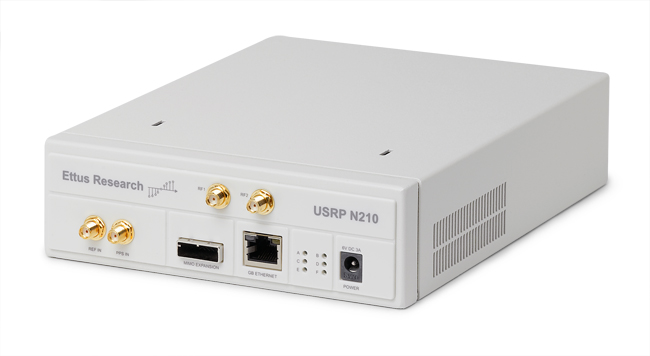
\includegraphics[width=0.90\textwidth]{includes/ettus_n210}
    \caption{USRP N210 Software Defined Radio}
	\label{fig:n210}
\end{figure}

\newpage
\item \textbf{Asterisk}\\
Um eine Gesprächsvermittlung im Mobilfunknetz realisieren zu können, wird ein Private Branch Exchange (PBX) oder SIP Softswitch wie Asterisk benötigt, welcher somit die Hauptfunktionen eines klassischen Mobile Switching Center (MSC) übernimmt. Asterisk bietet die Möglichkeit sowohl innerhalb des eigenen Mobilfunknetzes, als auch ins Festnetz und zu VoIP-Services, Gespräche aufzubauen und unterstützt weitere Features wie Sprachdienste, Mailbox-Services oder Telefonkonferenzen.

\item \textbf{SIPAuthServe}\\
SIPAuthserve verwaltet eine Subscriber Registry Datenbank, die die Teilnehmer-Informationen der im Netz registrierten Endgeräte enthält - unter anderem IMSI und Rufnummer. Diese Datenbank dient als Ersatz für das Home Location Register (HLR) eines klassischen GSM-Netzes sowie die SIP Registry von Asterisk.

\item \textbf{SMQueue}\\
SMQueue ist ein RFC-3428 Store-and-Forward Message Service für die Übertragung und Speicherung von SMS-Nachrichten. Es verfügt über einen Shortcode-Handler, welcher es ermöglicht den Inhalt von Textnachrichten als Eingabeargumente zu nutzen. So beinhaltet SMQueue standardmäßig einen Registrierungsprozess, der Benutzern dabei hilft eine gewünschte Rufnummer zu registrieren.
\end{itemize}

Die Beziehungen und Verbindungsprotokolle aller Komponenten eines OpenBTS-Systems werden in Abbildung\ref{fig:openbts} dargestellt. Dabei repräsentieren eckige Boxen Hardware-Komponenten, abgerundete Boxen Software-Komponenten.
\begin{figure}[htbp]
	\centering
		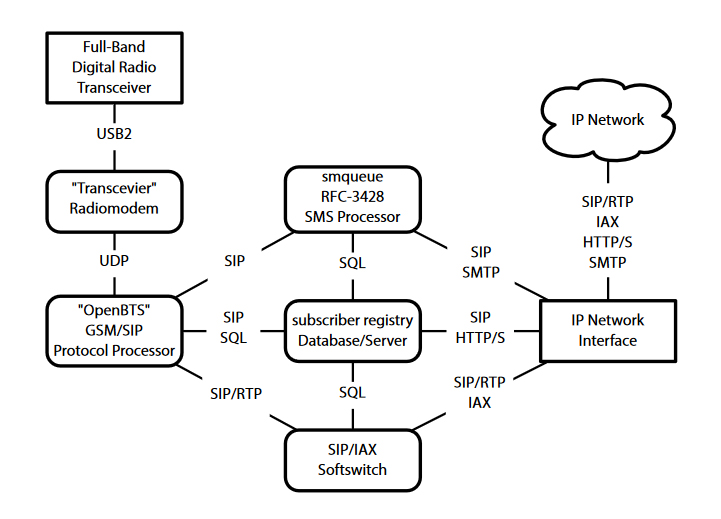
\includegraphics[width=1.00\textwidth]{includes/openbts}
	\caption{OpenBTS Systembestandteile}
	\label{fig:openbts}
\end{figure}

\newpage

\subsubsection{Datenbanken}
Da in OpenBTS viele unterschiedliche Software-Komponenten miteinander interagieren, werden auch mehrere Datenbanken für Einstellungen oder die Kommunikation zwischen verschiedenen Komponenten benötigt. Die folgenden Datenbanken kommen dabei zum Einsatz:

\begin{table}[h]
	\centering
		\begin{tabular}{ll}
			\textbf{OpenBTS.db} & Enthält alle Konfigurationseinstellungen des OpenBTS-Hauptprogramms.\\
			& Die Einstellungen der für uns lizenzierten Frequenz, sowie Netzwerk-\\
			& parameter wie MCC, MNC oder Name können hier gesetzt werden.\\
			\textbf{TMSITable.db} & Enthält die TMSI-IMSI Beziehungen der registrierten Endgeräte und wird\\
			& vom OpenBTS-Hauptprogramm genutzt. Der Pfad wird als Parameter in\\
			& der OpenBTS.db-Datenbank gesetzt.\\
			\textbf{ChannelTable.db} & Enthält den Channel Status aller aktiven Channel und wird vom OpenBTS-\\
			& Hauptprogramm genutzt. Der Pfad wird als Parameter in der OpenBTS.db-\\
			& Datenbank gesetzt.\\
			\textbf{sipauthserve.db} & Enthält alle Konfigurationseinstellungen von SIPAuthServe, unter anderem\\
			& den Dateipfad zur Subscriber Registry (sqlite3.db).\\
			\textbf{smqueue.db} & Enthält alle Konfigurationseinstellungen von SMQueue, unter anderem\\
			& den Dateipfad zur Subscriber Registry (sqlite3.db).\\
			\textbf{sqlite3.db} & Subscriber Registry, auf die von SIPAuthServe und SMQueue zugegriffen\\
			& wird. Wenn Asterisk mit Real-Time Funktionen konfiguriert wird, greift\\
			& auch Asterisk via ODBC auf die sqlite3-Datenbank zu.\\
		\end{tabular}
\end{table}

Der Kommunikationsfluss der OpenBTS-Komponenten über die Datenbanken ist in Abbildung \ref{fig:openbts_system_diagram} dargestellt. \textbf{Schwarze} Pfeile bezeichnen SIP-Verbindungen, \textcolor{red}{\textbf{rote}} Pfeile stellen Datenbankzugriffe dar und der \textcolor{blue}{\textbf{blaue}} Pfeil eine ODBC-Verbindung, die nicht standardmäßig in OpenBTS integriert ist und die zusätzlich für Asterisk Real-Time konfiguriert werden muss.
\begin{figure}[htbp]
	\centering
		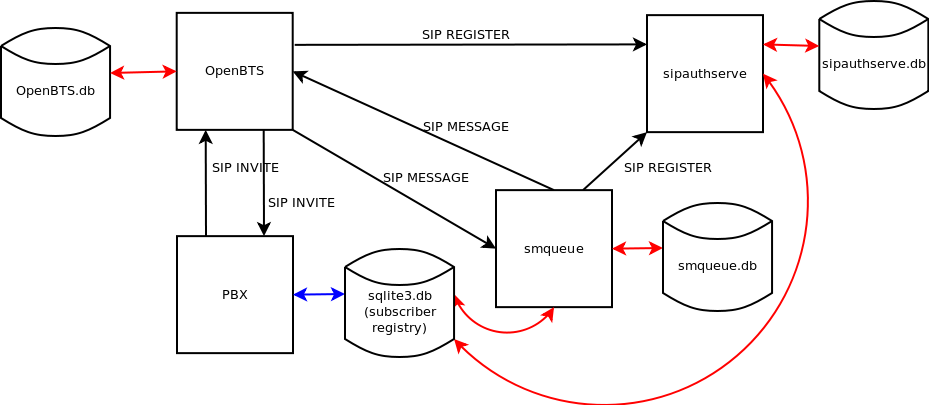
\includegraphics[width=1.00\textwidth]{includes/openbts_system_diagram}
	\caption{OpenBTS System Diagramm}
	\label{fig:openbts_system_diagram}
\end{figure}




\newpage
\subsection{}